\subsection{Ground-Launched Intercept}\label{sec:example-ground-intercept}

This problem simulates a ground-launched interceptor flying against a tactical
ballistic-missile target using the predictive guidance algorithm described in
\cref{sec:intercepts-pn}.  The target trajectory is computed
from an altitude of 200,000 ft to impact.  The interceptor launches 30 seconds after
the target trajectory begins; this time is selected so that the target lies within the
interceptor envelope.

\taossubhead{Problem File}

\lstinputlisting[style=taosmanual,basicstyle=\ttfamily\scriptsize]{examples/chapter04/ground-launched-intercept-source.prb.txt}

Trajectory 1 is the interceptor and trajectory 2 is the target.  The interceptor heads
east and the target heads west, as in the air-launched example.  Both trajectories
contain \problemblock{*dwn/crs} blocks so that the east and north output variables
share the same reference point.

The interceptor is rail launched and allowed to accelerate to 2500 ft/s before it
begins trying to intercept the target.  The $75^\circ$ launch angle is an estimated
value used simply to get the missile into the air.

The problem assumes constant interceptor thrust and mass flow, so the numbers are
entered directly in the \problemblock{*prop} blocks rather than being obtained from
tables.  This illustrates that a table value can be replaced by a constant for a simple
problem.

The \texttt{intercept=2} guidance rule in segments 3 and 4 maneuvers the
interceptor toward trajectory 2.  Within trajectory 1, \statevar{relvel[2]} is the
velocity of the target relative to the interceptor.  When this closing velocity changes
sign, the interceptor has reached its closest approach to the target.  Therefore,
\texttt{relvel[2]>0} is used as a final condition in both intercept segments.

Segment 3 also ends at \texttt{time>42}, representing motor burnout.  The value 42
may appear inconsistent with a 12-second burn until the interceptor initial time is
remembered: it launches at 30 seconds, so the burn duration is $42-30=12$ seconds.

\taossubhead{Results}

The source problem required approximately 1.5 seconds on a Silicon Graphics
workstation.  The interceptor printout is reproduced below:

\begin{center}
\begin{minipage}{0.98\linewidth}
\lstinputlisting[style=taosmanual,basicstyle=\ttfamily\tiny]{examples/chapter04/ground-intercept-printout.txt}
\end{minipage}
\end{center}

Predictive guidance begins with segment 3 at 37.059 seconds.  It immediately
commands a pitchover with negative angle of attack and then follows a nearly straight
path.  As the interceptor approaches the target, increasingly rapid corrections are
required.  At the end of the trajectory, angle of attack has reached its
$15^\circ$ limit.  The east-position and altitude histories are shown in
\cref{fig:example-ground-intercept}.

\begin{figure}[htbp]
  \centering
  \resizebox{0.84\linewidth}{!}{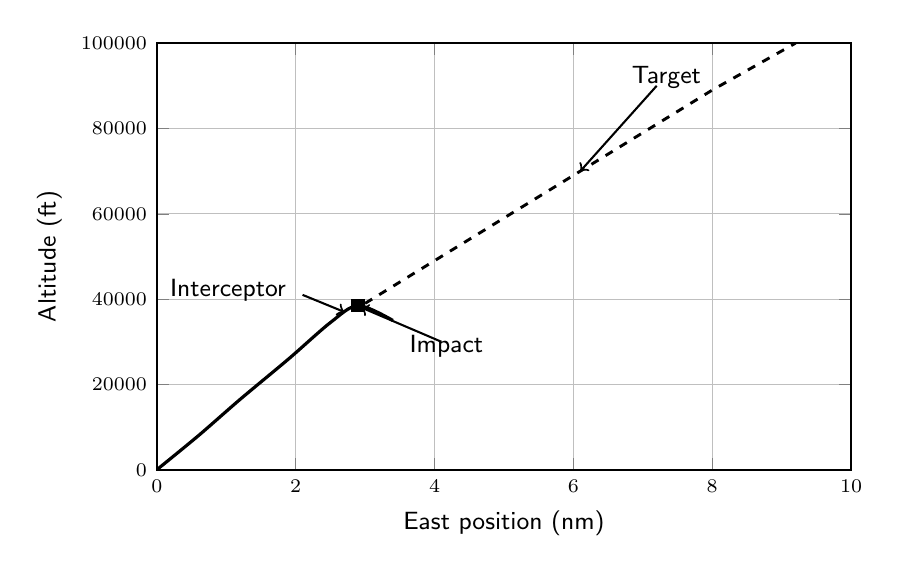
\begin{tikzpicture}
\begin{axis}[
  width=10.4cm,height=7.0cm,
  xmin=0,xmax=10,ymin=0,ymax=100000,
  xtick={0,2,4,6,8,10},
  ytick={0,20000,40000,60000,80000,100000},
  grid=major,
  axis line style={line width=0.8pt},
  tick label style={font=\scriptsize},
  label style={font=\sffamily\small},
  xlabel={East position (nm)},ylabel={Altitude (ft)},
  scaled y ticks=false,
  yticklabel style={/pgf/number format/fixed,/pgf/number format/1000 sep={}},
]
  \addplot[line width=1.15pt,smooth] coordinates {(0,0) (0.6,8000) (1.2,16500) (1.9,26000) (2.5,34500) (2.9,38500) (3.4,35000)};
  \addplot[line width=1.05pt,dashed] coordinates {(3.0,39000) (4.2,51000) (5.5,64000) (6.8,77000) (8.0,89000) (9.2,100000)};
  \addplot[only marks,mark=square*,mark size=2.2pt] coordinates {(2.9,38500)};
  \node[font=\sffamily\small,anchor=east] at (axis cs:2.0,42000) {Interceptor};
  \draw[->,line width=0.75pt] (axis cs:2.1,41000)--(axis cs:2.7,37000);
  \node[font=\sffamily\small,anchor=west] at (axis cs:6.7,92000) {Target};
  \draw[->,line width=0.75pt] (axis cs:7.2,90000)--(axis cs:6.1,70000);
  \node[font=\sffamily\small,anchor=west] at (axis cs:3.5,29000) {Impact};
  \draw[->,line width=0.75pt] (axis cs:4.1,30000)--(axis cs:2.95,38000);
\end{axis}
\end{tikzpicture}
}
  \caption{Ground-launched intercept example.}
  \label{fig:example-ground-intercept}
\end{figure}
